\documentclass{article}
\usepackage[utf8]{inputenc}
\usepackage{graphicx}
\setlength{\voffset}{-0.85in}
\setlength{\headsep}{1pt}
\usepackage[headsep=0pt]{geometry}

\usepackage{caption}
\usepackage{subcaption}
\title{Solving ConnectN}
\author{Vlad Stelea, Connor Mclaughlin, Will Lucca}
\date{February 2020}

\begin{document}

\maketitle

\section{Problem Statement}
Most people are familiar with the game Connect4, a game where you place pieces on a board with the objective of putting 4 symbols in a row. Our task is to not only devise an AI agent using alpha-beta-pruning for Connect4, but a variable-objective game, ConnectN. 

\section{Our Approach}
Our agent uses a minimax algorithm with alpha-beta pruning to evaluate potential moves and decide what to do. It uses three different heuristic functions that are weighted individually to find the utility of potential board states. We also utilized a genetic algorithm to train the weights of these heuristics by playing different alpha-beta agents against each other.

\section{Finding Heuristics}
In order to determine our heuristics, we identified key board states that we wanted our alpha-beta minimax function to maximize the chances of reaching. We then implemented detection of these states with basic heuristic functions. The total utility of any board state is the sum of the heuristic values multiplied by their respective weights. In order to determine the best heuristic weights, we designed a genetic algorithm that trained the weights of the heuristics.

\subsection{The Heuristic Functions}
Early on in the design of our algorithm, we tackled the heuristics problem with three evaluation functions for different board states.

\subsubsection*{The Adjacency Heuristic}
The Adjacency Heuristic increases in value as more friendly tokens are bordering each other, adjacently or diagonally. Each token is worth points equal to its number of neighbors, and the total heuristic value is equal to the sum of these points.

\begin{figure}[h]
  \centering
  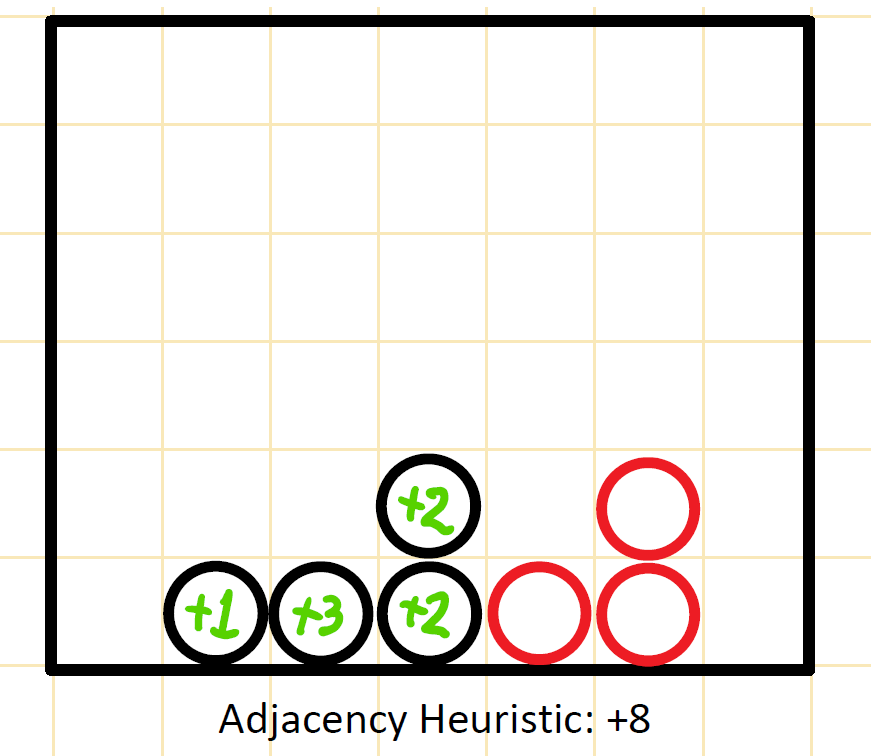
\includegraphics[width=0.45\linewidth]{Writeup/adj-util.jpg}
  \captionsetup{labelformat=empty}
  \captionof{figure}{For the black player: the token on the left has one neighbor, the token in the middle has three, etc.}
  \label{fig:test1}
\end{figure}

\subsubsection*{The Opportunity Heuristic}
The Opportunity Heuristic increases in value the more “chains” (i.e. lines of tokens shorter than n) of friendly tokens exist. Each chain is worth points equal to its length squared, therefore rewarding longer chains that are closer to victory with exponentially more value. A chain only counts if the player could have the opportunity to make it into an n-in-a-row line. If n-in-a-row cannot be formed because it is blocked by the end of the board or by the opponent’s tokens, the chain earns no points during evaluation.

\begin{figure}[htb]
    \centering
    \begin{subfigure}[b]{\textwidth}
        \centering
        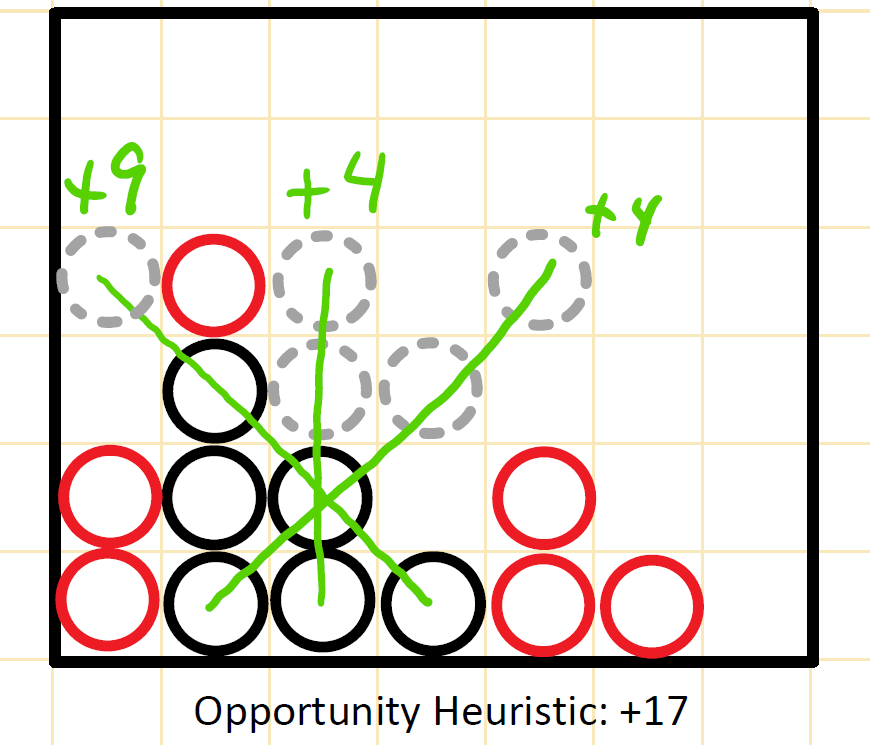
\includegraphics[width=0.45\linewidth]{Writeup/opp-util-1.jpg}%
        \hfill
        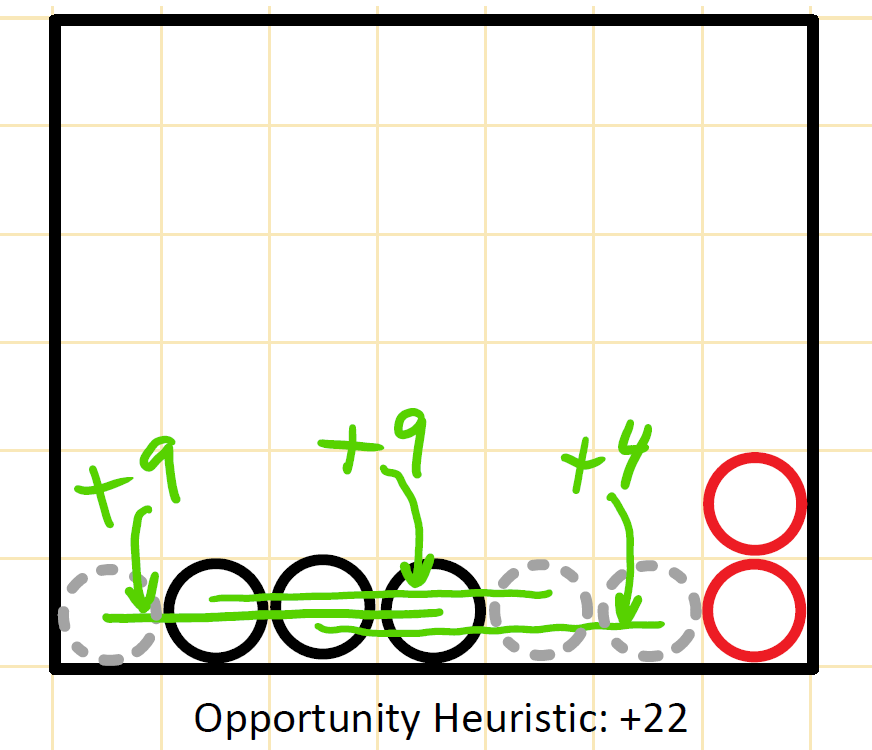
\includegraphics[width=0.45\linewidth]{Writeup/opp-util-2.jpg}
        \captionsetup{labelformat=empty}
        \caption{While there can be many chains of length 2 or 3, only the ones with the potential to become 4-in-a-row are awarded points (left board). A single token can be a part of multiple 4-in-a-row chains (right board).}
    \end{subfigure}
\end{figure}

\subsubsection*{The Is Completed Game Heuristic}
The Is Game Completed Heuristic returns an extremely positive utility with a winning board, an extremely negative utility with a losing board, or 0 with an incomplete or tied game board. While the previous heuristic checked for potential winning moves in a given state, this function only provides points for the win or lose states themselves.

\begin{figure}[htb]
    \centering
    \begin{subfigure}[b]{\textwidth}
        \centering
        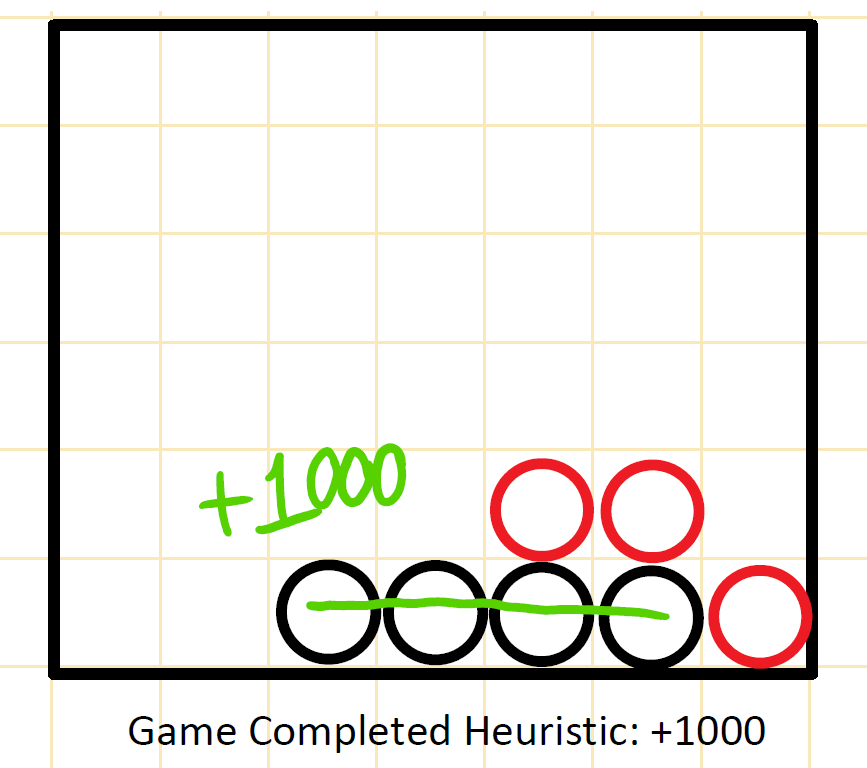
\includegraphics[width=0.45\linewidth]{Writeup/win-util-1.jpg}%
        \hfill
        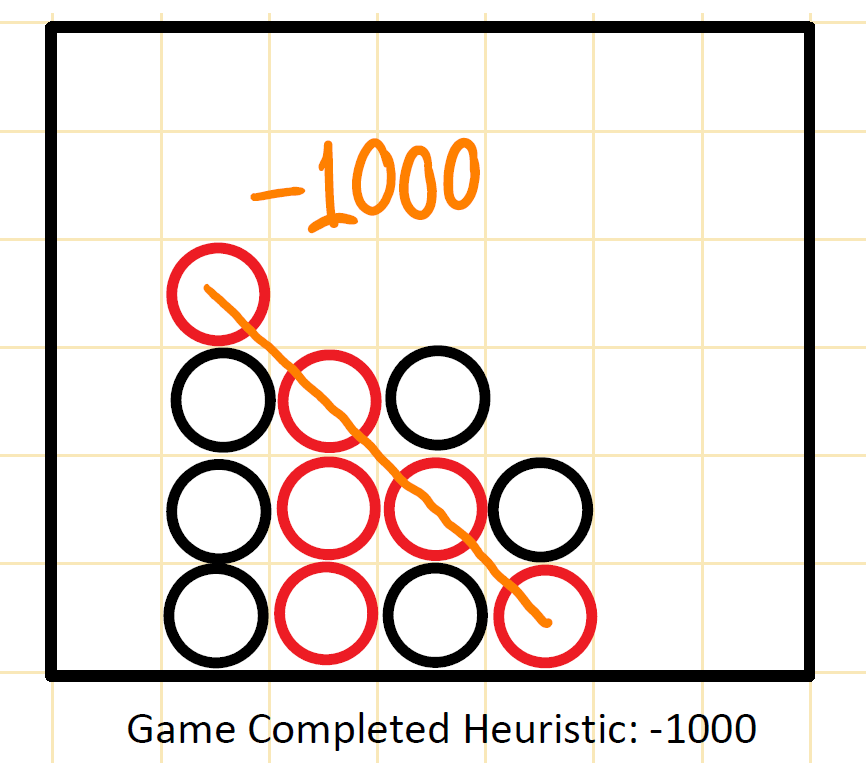
\includegraphics[width=0.45\linewidth]{Writeup/win-util-2.jpg}
        \captionsetup{labelformat=empty}
        \caption{This heuristic only returns a non-zero utility for a winning outcome (left) or a losing outcome (right), without considering any other factors about the board.}
    \end{subfigure}
\end{figure}

\section{Optimizing the Heuristics}
In order to optimize the weighting of our heuristic values, we implemented a genetic algorithm. We decided to do a genetic algorithm as the selection process of playing matches against itself was the most natural way to evaluate the quality of our heuristic weights. The genotype consisted of a tuple of floating-point multipliers to the initial heuristic values in the format: (adjacency\textunderscore heuristic, opportunity\textunderscore heuristic, game\textunderscore complete heuristic). We chose a population size of 16, and we initialized the genotypes for the starting population with random values from [-1, 1] for each gene.

We took these individuals and ran them in a pooled tournament. With each generation, we would break them into a certain number of pools (in our case, we settled on 4). In each of these smaller groups, each player would play all of the other players in a round-robin fashion. After each individual within a pool had played against each other, we stored the individual with the most wins. Afterward, we took the winners from each pool and put them in one final round-robin tournament, this time only taking the best two. These individuals became the parents for the next generation and the loop repeated. We chose this tournament format over a simple round-robin of 16 individuals as it greatly reduced the number of games played per generation (and in doing so, our runtime) without sacrificing too much quality. 

We initially tested our genetic algorithm with 100 generation-runs, but soon increased it to 300 generations per training. We did this because we saw that the 100 generation-runs were leaving us with inconsistent results, and more generations would give it a chance to mutate more and try more things, and converge to a higher quality solution. 

\section{Results}
After running our genetic algorithm, we discovered how best to weigh the importance of each of our heuristics.

The feedback on the adjacency heuristic was the most interesting of the three. We saw individuals that succeeded with both positive scale factors (in the range 0.5 to 0.8) as well as individuals which associated a small negative scale factor to the adjacency heuristic (in the range -0.1 to -0.5). After further manual testing of these individuals, it seems as though those who valued placing tiles closer together were more successful when they had the first move of the game, and those who were averse to the adjacency heuristic had more success when they were second to move.  
When it came to Connect5, however, all of the individuals we saw seemed to value the adjacency heuristic (values in range 0.7 to 0.9).

In a less surprising manner, all of the individuals prioritizes the opportunity and game\textunderscore completed utilities very highly (0.7 to 1.3).

\section{Reflection}
One potential change we could have made would have tried using the binary representation of our scale factors as our genotype, as opposed to simply a tuple of floats. A bit-wise crossover might have enabled a more productive process of mutation/splicing, which could have improved our results from the genetic algorithm. 


\end{document}
